\documentclass{beamer}
\mode<presentation>
{
  %\usetheme{}
  %\usecolortheme{beaver}
  % 可供选择的主题参见 beameruserguide.pdf, 第 134 页起
  % 无导航条的主题: Bergen, Boadilla, Madrid, Pittsburgh, Rochester;
  % 有树形导航条的主题: Antibes, JuanLesPins, Montpellier;
  % 有目录竖条的主题: Berkeley, PaloAlto, Goettingen, Marburg, Hannover;
  % 有圆点导航条的主题: Berlin, Dresden, Darmstadt, Frankfurt, Singapore, Szeged;
  % 有节与小节导航条的主题: Copenhagen, Luebeck, Malmos, Warsaw
  %\setbeamercovered{transparent}
  % 如果取消上一行的注解 %, 就会使得被覆盖部分变得透明(依稀可见)
} 
\definecolor{kugreen}{RGB}{160,63,171}
\definecolor{kugreenlys}{RGB}{132,158,139}
\definecolor{kugreenlyslys}{RGB}{173,190,177}
\definecolor{kugreenlyslyslys}{RGB}{214,223,216}
\setbeamercovered{transparent}
\mode<presentation>
{  
  \usetheme{PaloAlto}
  \usecolortheme[named=kugreen]{structure}
  \useinnertheme{circles}
  \usefonttheme[onlymath]{serif}
  \setbeamercovered{transparent}
  \setbeamertemplate{blocks}[rounded][shadow=true]
}

\usepackage[english]{babel}
\usepackage{multirow}
\usepackage{amsmath}
\usepackage{amsfonts}
\usepackage{xkeyval}
\usepackage{graphics}
\usepackage{url}
\usepackage[lined,boxed,linesnumbered]{algorithm2e}

\logo{
\includegraphics[scale=0.08]{images/HUSTLogo}}%Logo of the presentation
\title{Robust classification using $\ell_{2,1}$-norm based regression model}  
\author{Yunfei Wang}
\institute{Department of Computer Science \& Technology \\ Huazhong University of Science \& Technology}
\date{\today} 

\begin{document}

\begin{frame}
\titlepage
\end{frame}


\begin{frame}\frametitle{Table of contents}
\tableofcontents
\end{frame}


\section{Main Algorithm using $\ell_{2,1}$-norm based regression}
\subsection{Basic Regression Model}
\begin{frame}\frametitle{Basic Regression Model}
$N$ test samples:$Y=[y_1,y_2,\cdots ,y_N]\in \mathbb{R}^{d \times N}$\\
$n$ training samples:$A=[a_1,a_2,\cdots ,a_n]\in \mathbb{R}^{n \times d}$\\
We aim to obtain a coefficient matrix $X\in \mathbb{R}^{n \times N}$ such that
\begin{displaymath}
Y \approx A^TX
\end{displaymath}
This formulation actually indicates that the combination of training samples will be used to approximate each sample.
\end{frame}

\subsection{Objective criterion as a constrained problem}
\begin{frame}\frametitle{Properties of $\ell_{2,1}$-norm}
The $\ell_{2,1}$-norm is defined as
\begin{displaymath}
\|A\|_{2,1}=\sum_{i=1}^j\sqrt{\sum_{j=1}^m a_{ij}^2}=\sum_{i=1}^n\|a_i\|^2
\end{displaymath}
\begin{itemize}
\item Decrease the negative impact of outliers to which $\ell_2$-norm is fairly sensitive.
\item Rotational invariant\\
For any orthogonal matrix $R$ and data transformation:$x_i=R x_i$,the $\ell_{2,1}$-norm is invariant $\|x_i\|_{2,1}=\|R x_i\|_{2,1}$.
\end{itemize}
\end{frame}

\begin{frame}\frametitle{Minimizing Loss}
Here we use $\ell_{2,1}$-norm as a criterion to evaluate approximation:
\begin{equation}\label{eq:obj1}
arg \min_X J(X)=\|A^TX-Y\|_{2,1}
\end{equation} 
in which $X=[x_1,x_2,\cdots ,x_N]$ is the representation matrix and $x_i\in \mathbb{R}^n(i=1,2,\cdots ,N)$ is the representation of test sample $y_i$ using the entire training samples.
\end{frame}

\begin{frame}\frametitle{Adding regularization term}
The $\ell_{2,1}$-norm regularization term $R(x)$ with a parameter $\rho$ is performed to select class-specific samples with some \textcolor{red}{sparsity}.
$R(X)=\|X\|_{2,1}$ and $\rho$ is the penalty coefficient,the regularized form of Eq.(\ref{eq:obj1}) is equivalent to
\begin{equation}\label{eq:obj2}
\begin{split}
arg \min_X J(X)+\rho R(X)&=arg \min_X\|A^TX-Y\|_{2,1}+\rho \|X\|_{2,1}\\
&=arg \min_X \frac{1}{\rho}\|A^TX-Y\|_{2,1}+\|X\|_{2,1}
\end{split}
\end{equation}
\end{frame}

\begin{frame}\frametitle{Reformulating the Objective function}
Suppose $E=\frac{1}{\rho}(Y-A^TX)$,$B=(A^T,\rho I)$ and $U=\left(\begin{array}{c}X\\E\end{array}\right)$
\begin{equation}\label{eq:obj3}
\begin{split}
&\frac{1}{\rho}\|A^TX-Y\|_{2,1}+\|X\|_{2,1}\\
&=\|E\|_{2,1}+\|X\|_{2,1}\\
&=\left\Vert\begin{array}{c}X\\E\end{array}\right\Vert_{2,1}\\
&=\|U\|_{2,1}
\end{split}
\end{equation}
subject to $A^TX+\rho E=Y$.\\
Finally,the objective criterion can be formulated as
\begin{equation}\label{eq:obj4}
U^*=arg \min_U \vert U\vert_{2,1}\;s.t.\;BU=Y
\end{equation}
\end{frame}

\begin{frame}\frametitle{Solving the optimization problem}
An efficient algorithm was proposed to solve this specific problem,in which gradient-descent approach is implemented on the Lagrangian function to obtain the iterative solution
\begin{equation}\label{eq:opt}
U=D^{-1}B^T(BD^{-1}B^T)^{-1}Y
\end{equation}
in which $D$ is a diagonal matrix with the i-th diagonal element as $d_{ii}=\frac{1}{2\|u_i\|^2}$\\
Usually,the matrix $BD^{-1}B^T$ is added by a diagonal matrix $\zeta I$ to avoid the singular problem,where $\zeta$ is a very small positive constant and $I$ is the unit matrix.
\begin{block}{Reference}
F.Nie,H. Huang,X. Cai,C. Ding.Efficient and robust feature selection via joint $\ell_{2,1}$-norm minimization,in:Twenty-Fourth Annual Conference on Neural Information Processing Systems,2010.
\end{block}
\end{frame}


\subsection{Classification Tactics}
\begin{frame}\frametitle{Classification Tactics}
\begin{enumerate}
\item Extracting the optimal representation $\hat{X}$(the first $n$ rows of matrix $U^*$).
\item Define $C$ functions $\delta_s$ to select only those $\hat{x}$ that correspond to class $s$,where $\hat{x}$ is the representation for the test sample $y$.
\item Approximation in terms of the coefficients associated with the sth class is $\hat{y}=A^T\delta_s(\hat{x})$.
\item Assign y to the class that minimizes $\|y-A^T\delta_s(\hat{x})\|_2$
\end{enumerate}
\end{frame}

\begin{frame}\frametitle{Pseudo-code of the algorithm}
\begin{algorithm}[H]
\KwIn{$A \in \mathbb R^{n \times d},Y \in \mathbb R^{d \times N},\rho$;}
\KwOut{ID(Y);}
\emph{Set $B=\left[ A^T,\rho I \right],t=0$}\;
\emph{Initialize $D_t \in \mathbb R^{(n+d) \times (n+d)}$ as an identity matrix}\;
\Repeat(\tcp*[h]{Iteratively compute U}){Convergence}
{
	Calculate $U_{t+1}=D_t^{-1}B^T(BD_t^{-1}B^T)^{-1}Y$\;
	Calculate the diagonal matrix $D_{t+1}$,where the i-th diagonal element is $\frac{1}{2\|u_{t+1}^t\|_2}$\;
	$t=t+1$\;
}
\For{$j= 1$ \KwTo $N$}
{
	Get $r_s(y_j)=\|y-A^T\delta_s(x_j)\|_2,s=1,2,\cdots ,C$\;
	$ID(y_i)=\mathop{\min}\limits_{s=1,2,\cdots ,C}r_s(y_j)$\;
}
\Return $ID(Y)=((ID(y_1),ID(y_2),\cdots ,ID(y_n))$\;	
\caption{Classification using $\ell_{2,1}$-norm based regression model}
\end{algorithm}
\end{frame}

\begin{frame}\frametitle{Experiment results of RRC}
Classification accuracy on 4 datasets:Yale,YaleB,COIL and ORL.
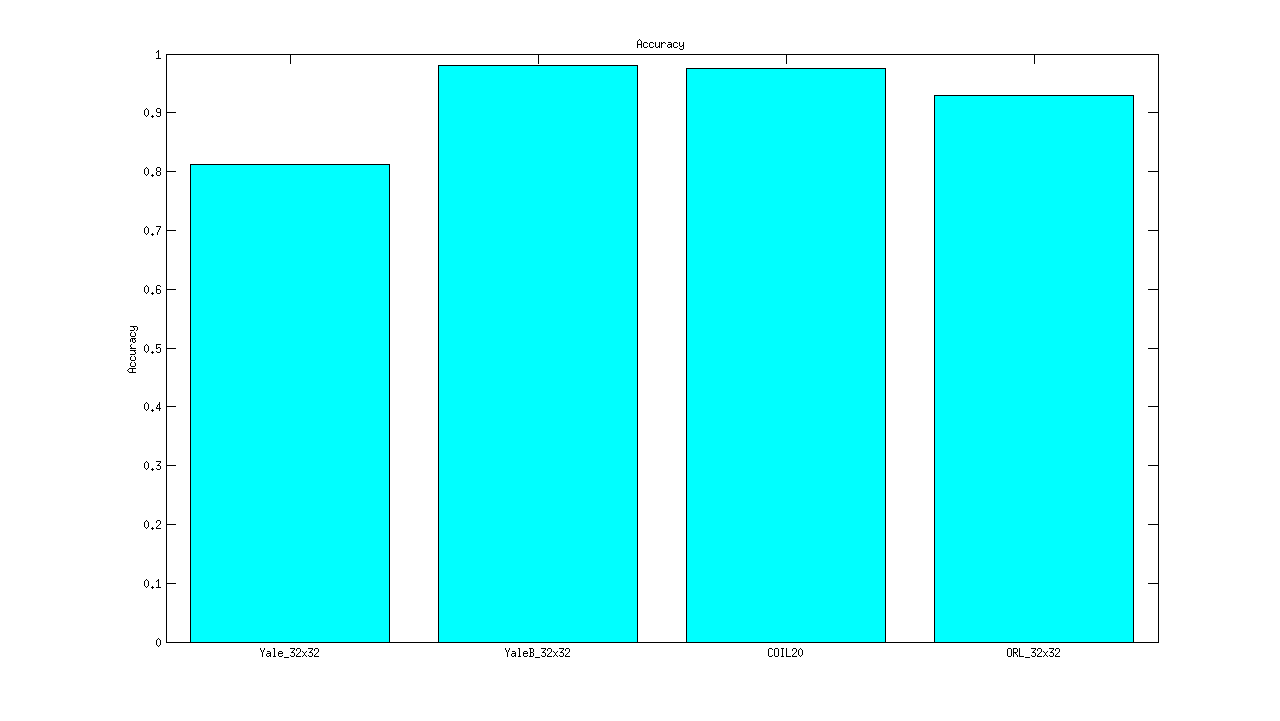
\includegraphics[scale=0.3]{images/accuracy}
\end{frame}
\end{document}
